\appendix
\chapter*{Annexe}
\addcontentsline{toc}{chapter}{Annexe}
\renewcommand{\thesection}{A.\arabic{section}}


\begin{landscape}
\section{Statistiques du repository Github}
\label{Statistiques du repository Github}
\begin{center}
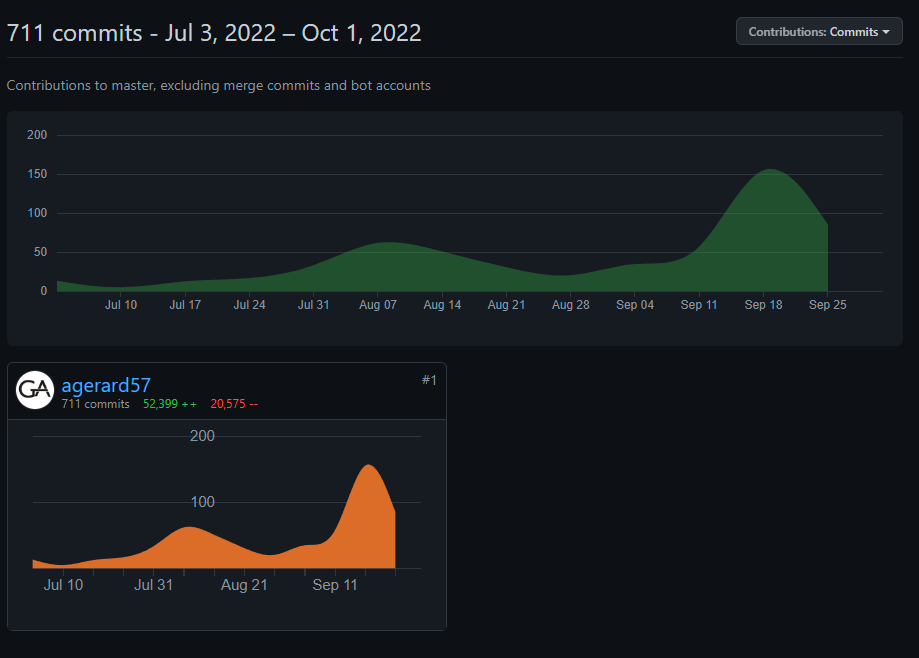
\includegraphics[scale=0.8]{medias/commits.png}
\end{center}
\end{landscape}

\begin{landscape}
\section{CORS S3}
\label{CORS S3}
\begin{center}
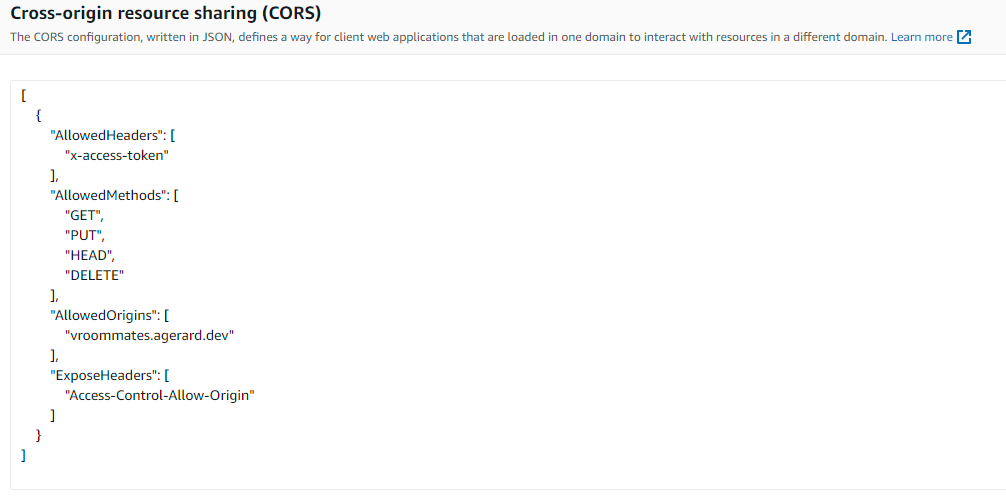
\includegraphics[scale=0.6]{medias/s3Cors.png}
\end{center}
\end{landscape}

\begin{landscape}
\section{Permissions IAM}
\label{Permissions IAM}
\begin{center}
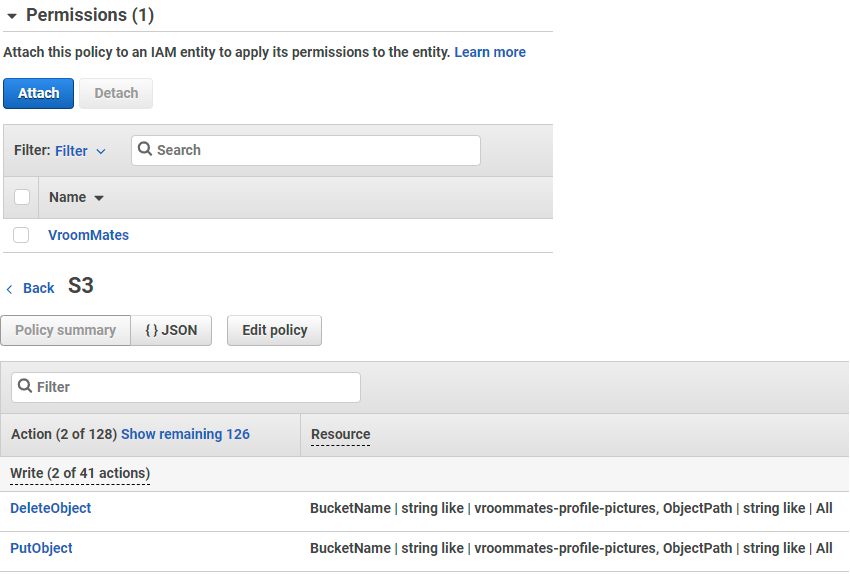
\includegraphics[scale=0.5]{medias/permissionsIAM.png}
\end{center}
\end{landscape}

\section{Diagramme de séquence: JWT}
\label{Diagramme de séquence: JWT}
\begin{center}
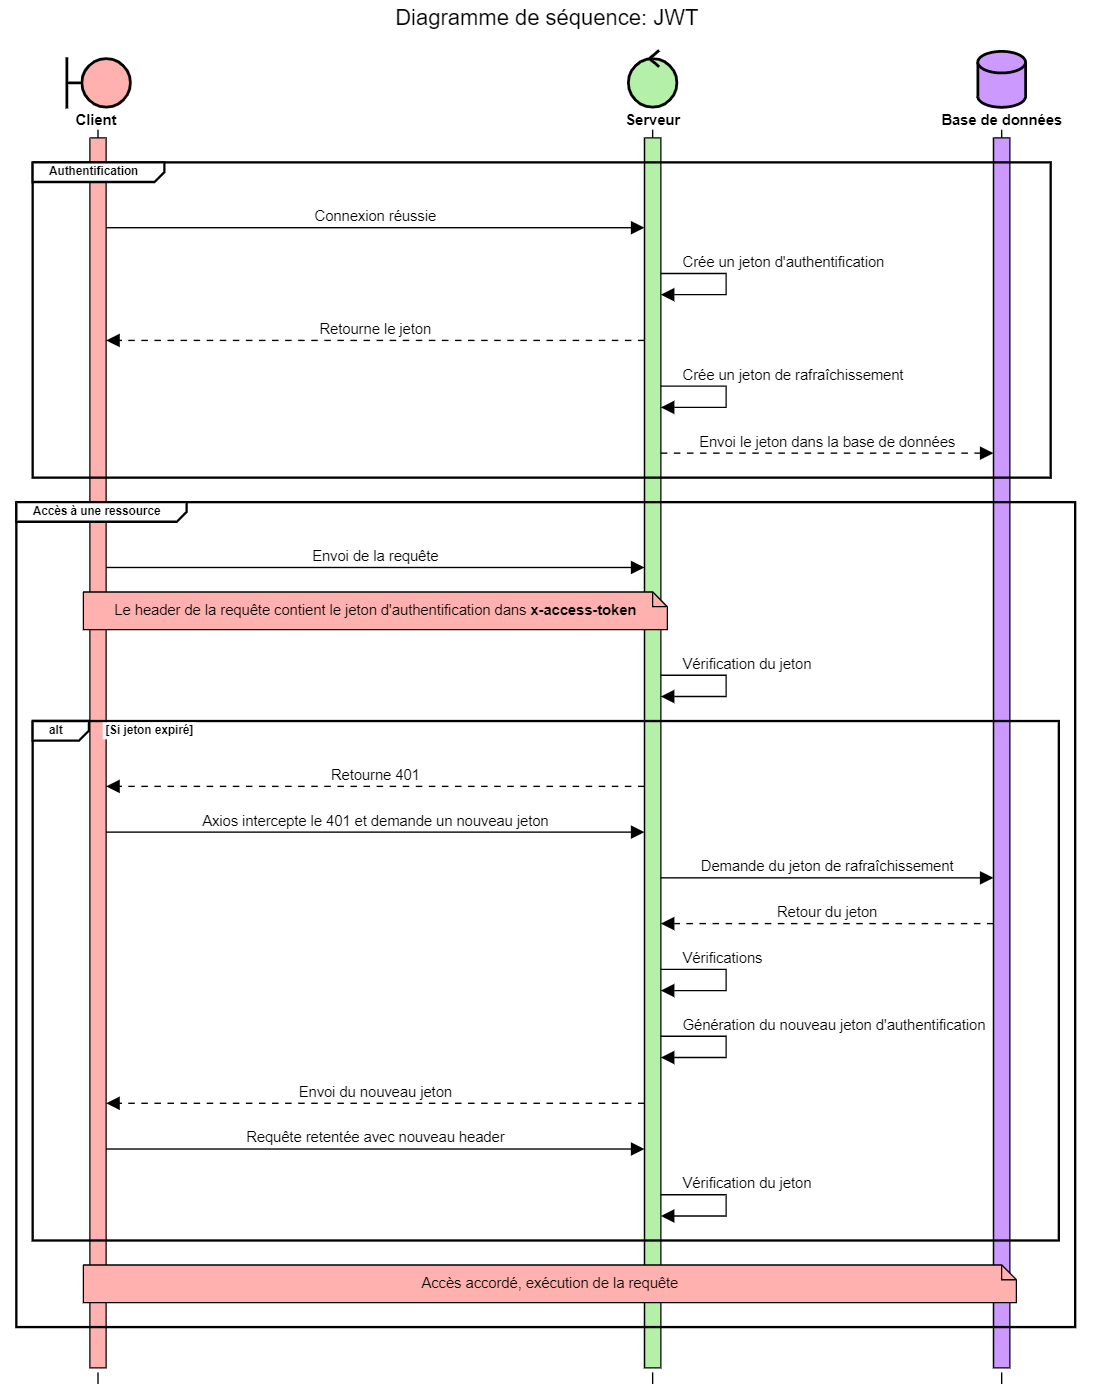
\includegraphics[width=\linewidth]{medias/diagrammeJWT.png}
\end{center}

\section{Exemple d'un cahier de recettes (landing page)}
\label{Exemple d'un cahier de recettes (landing page)}
\begin{center}
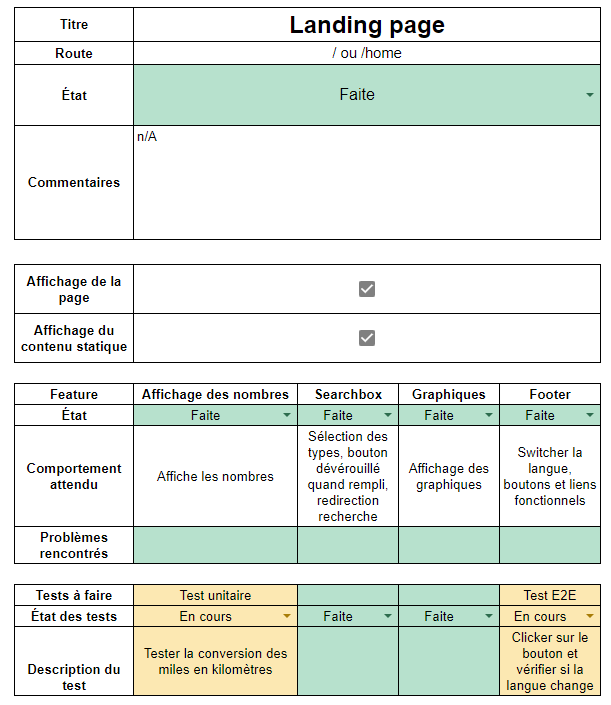
\includegraphics[width=\linewidth]{medias/cahierRecette.png}
\end{center}

\section{Exemple d'un schéma de validation (Drivers)}
\label{Exemple d'un schéma de validation (Drivers)}
\begin{center}
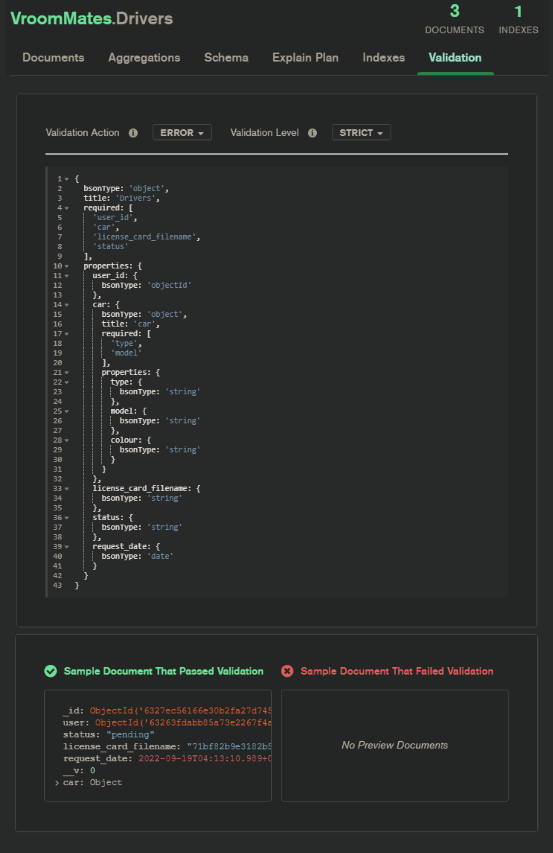
\includegraphics[width=\linewidth]{medias/validation.png}
\end{center}

\section{Structure de client et de server}
\label{Structure de client et de server}
\begin{center}
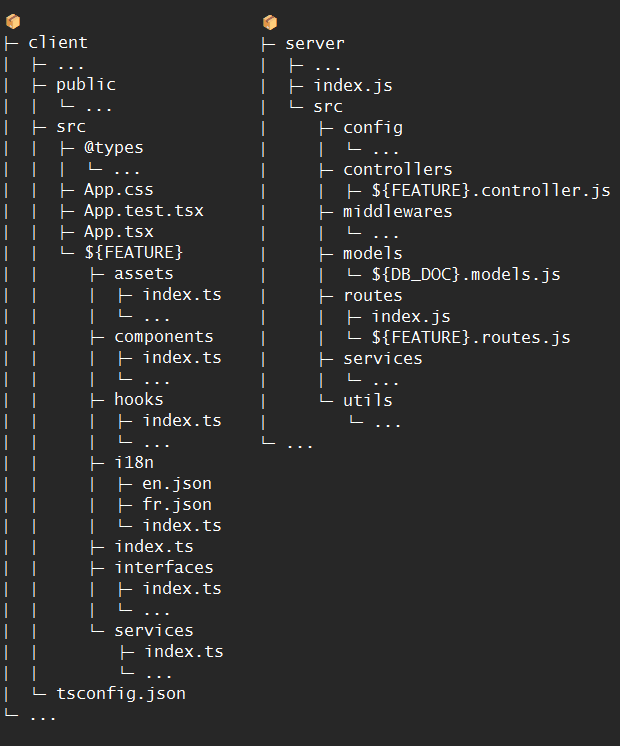
\includegraphics[width=\linewidth]{medias/structure.png}
\end{center}